%% =============================================================================
%% Appendix L — Technical & Operational Specifications
%% Houses the operational-engineering content moved out of Chapter 5
%% (Discussion) per 2026-05-12 brutal-feedback scoping discipline.
%%
%% Rationale: Chapter 5 is interpretive discussion; full operational-protocol
%% and engineering-specification content is non-contribution material per the
%% locked DBA identity ("human-centered Responsible AI governance research,
%% not engineering thesis"). This appendix is the proper home for:
%%   L1. Operational Compliance Gap Assessment (8 compliance domains)
%%   L2. Incident Response & Business Continuity Protocol
%%   L3. KPI Threshold-to-Action Escalation Protocol
%%   L4. Unified KPI Dashboard (15 operational KPIs)
%% Chapter 5 retains one-paragraph pointers to each section here.
%% =============================================================================

\addcontentsline{toc}{section}{Appendix L Framing} % [TOC-appendix-section-insertion]
\section*{Appendix L Framing}
\addcontentsline{toc}{section}{Appendix L Framing}
\label{sec:appl_framing}

\noindent\textbf{What this appendix is.} The operational-engineering and protocol-level
specifications that operationalise the governance contracts in the dissertation. Each
section was relocated from Chapter~5 (Discussion) to clarify the locked DBA identity:
Chapter~5 interprets the empirical findings and discusses managerial implications, while
this appendix specifies the operational protocols that a provider organisation would
implement when adopting the framework.

\noindent\textbf{What this appendix is not.} It is not the dissertation's contribution.
It is the operational-support layer (along with Appendix~H for architecture) that any
provider would need to instantiate the framework. Inclusion here is for completeness and
defensibility; absence from Chapter~5 reflects scope discipline.

\noindent\textbf{Cross-references retained.} Internal labels (e.g., \texttt{tab:compliance\_\allowbreak summary},
\texttt{tab:kpi\_\allowbreak dashboard}, \texttt{tab:kpi\_\allowbreak escalation}) are preserved unchanged so that
references from Chapter~5 and other appendices resolve to their original targets.

\paragraph{Appendix L Scope Contract --- Conceptual Future Reference Only.}
\label{para:appendix_l_scope_contract}
The operational and protocol-level specifications in this appendix (compliance gap assessment, incident-response protocols, KPI escalation thresholds, operational dashboards) are presented strictly as \textbf{conceptual future reference specifications, NOT as validated operational evaluation evidence}. Specifically: (i)~the compliance domains are \emph{conceptual governance alignment} (NIST AI RMF, ISO~42001, EU AI Act, HIPAA, GDPR, SOC~2), not audit-grade compliance certifications --- formal certification under each regulation requires separate audit, legal review, and regulator-specific evidence packages that are out of scope; (ii)~the incident-response and KPI-threshold protocols are \emph{operational design templates} that provider organisations would adapt to their own evaluation context, not validated runbook evidence from a deployed conceptual operational reference; (iii)~the operational dashboards are \emph{specification artefacts} showing what monitoring infrastructure would track in a hypothetical deployment, not live monitoring data from any operational system. The DBA contribution is the governance + explainability + adoption framework in Chapter~\ref{chap:discussion}; Appendix~L is operational scaffolding for that framework if adopted, not the contribution itself.


%% ======================================================================
%% L1. Operational Compliance Gap Assessment
%% Moved from Chapter 5 — 2026-05-12
%% ======================================================================
\addcontentsline{toc}{section}{L1. Operational Compliance Gap Assessment} % [TOC-appendix-section-insertion]
\section*{L1. Operational Compliance Gap Assessment}
\addcontentsline{toc}{section}{L1. Operational Compliance Gap Assessment}
\label{sec:appl_compliance}

Eight operational compliance domains are assessed in Appendix~\ref{chap:appendix_ch5} (Tables~E.2--E.9). Table~\ref{tab:compliance_summary} summarises readiness: 3 of 48 requirements fully implemented, 11 partial, 34 specified with KPIs.

\iffalse
%% APPENDIX CONTENT: Eight compliance domain tables (moved to Appendix E)
%% --- TABLE 1: PATIENT CONSENT & DATA SUBJECT RIGHTS ---
\needspace{24\baselineskip}
\begin{table}[H]
\tablestripes
\tablefontsize
\caption[Patient Consent and Data Subject Rights Assessment]{Domain~1: Patient Consent and Data Subject Rights --- Operational Compliance Assessment}
\begin{tabularx}{\textwidth}{@{} p{0.4cm} p{2cm} p{1.4cm} L L p{1.8cm} @{}}
\toprule
\thead{\#} & \thead{Requirement} & \thead{Status} & \thead{Input $\to$ Process $\to$ Output} & \thead{Decision Trigger} & \thead{KPI} \\
\midrule
1 & Informed consent & Partial & Data use agreements $\to$ IRB exemption review (45~CFR~46.104) $\to$ Exemption letter on file & Reject dataset without valid consent documentation & 100\% datasets with valid DUA \\
\addlinespace
2 & Right to erasure (GDPR Art.~17) & Specified & Erasure request $\to$ Data inventory scan + model impact assessment $\to$ Confirmation of deletion + retraining trigger & Mandatory response within 30 days of DSAR receipt & DSAR response time $\leq$30 days \\
\addlinespace
3 & Right to explanation (GDPR Art.~22) & Partial & Automated prediction $\to$ RAG explanation generation $\to$ Literature-grounded rationale & Provide explanation for every automated decision affecting patients & 100\% predictions with explanations \\
\addlinespace
4 & Consent withdrawal & Specified & Withdrawal request $\to$ Subject data identification + removal + model impact assessment $\to$ Acknowledgement + data purge & Immediate halt of data processing for withdrawn subjects & Withdrawal processing $\leq$72 hours \\
\addlinespace
5 & Data portability (GDPR Art.~20) & Specified & Portability request $\to$ Data extraction in machine-readable format $\to$ Structured export (JSON/CSV) & Export provided within 30 days of request & Portability request fulfilment $\leq$30 days \\
\addlinespace
6 & Opt-out mechanism & Specified & Patient opt-out $\to$ Consent registry update + data flagging $\to$ Exclusion from future processing & Opt-out processed before next batch cycle & Opt-out processing $\leq$24 hours \\
\bottomrule
\end{tabularx}
\vspace{0.5em}\noindent\textit{Note.} Status: \textit{Implemented} = operational; \textit{Partial} = mechanism exists, not conceptual operational reference (not validated production); \textit{Specified} = protocol defined with SLAs (Table~\ref{tab:consent_protocol}). DSAR = data subject access request; DUA = data use agreement; GDPR = General Data Protection Regulation; IRB = Institutional Review Board.
\end{table}

%% --- TABLE 2: REGULATORY COMPLIANCE & SUBMISSION READINESS ---
\needspace{24\baselineskip}
\begin{table}[H]
\tablestripes
\tablefontsize
\caption[Regulatory Compliance and Submission Readiness]{Domain~2: Regulatory Compliance and Submission Readiness --- Operational Compliance Assessment}
\begin{tabularx}{\textwidth}{@{} p{0.4cm} p{2cm} p{1.4cm} L L p{1.8cm} @{}}
\toprule
\thead{\#} & \thead{Requirement} & \thead{Status} & \thead{Input $\to$ Process $\to$ Output} & \thead{Decision Trigger} & \thead{KPI} \\
\midrule
1 & FDA SaMD classification & Partial & Clinical intent + risk level $\to$ SaMD classification (Class~II) $\to$ Regulatory strategy document & Pre-submission meeting with FDA before pilot & Classification confirmed within 90 days \\
\addlinespace
2 & EU AI Act high-risk registration & Partial & System risk assessment $\to$ Conformity assessment (Art.~43) $\to$ CE marking documentation & Registration before EU market entry & Conformity assessment completion \\
\addlinespace
3 & 21~CFR Part~11 (e-records) & Specified & Digital signatures + audit logs $\to$ Validation of electronic record integrity $\to$ Part~11 compliance report & All e-records meet Part~11 before FDA submission & 100\% e-records validated \\
\addlinespace
4 & Post-market surveillance & Specified & Real-world performance data $\to$ Adverse event detection + trend analysis $\to$ Periodic safety update report & Adverse event reported within 15 days (MDR timeline) & Adverse event detection rate \\
\addlinespace
5 & Clinical evaluation report & Specified & Literature review + clinical data + performance evidence $\to$ Structured CER per MEDDEV 2.7/1 $\to$ CER document for regulatory body & CER updated annually or upon significant change & CER currency $\leq$12 months \\
\addlinespace
6 & HIPAA technical safeguards & Partial & PHI inventory + risk assessment $\to$ Encryption + access controls + audit logging $\to$ HIPAA compliance attestation & Annual compliance attestation required & 100\% technical safeguards implemented \\
\bottomrule
\end{tabularx}
\vspace{0.5em}\noindent\textit{Note.} SaMD = Software as a Medical Device; CER = Clinical Evaluation Report; MEDDEV = European Medical Device Guidance; MDR = Medical Device Regulation; PHI = protected health information. Current framework maps governance to regulatory requirements; submission-ready documentation requires 12--18 months of additional preparation.
\end{table}

%% --- TABLE 3: PII & DATA PROTECTION ---
\needspace{24\baselineskip}
\noindent The table below presents the domain~3: PII and Data Protection --- Operational Compliance Assessment.

\begin{table}[H]
\tablestripes
\tablefontsize
\caption[PII and Data Protection Assessment]{Domain~3: PII and Data Protection --- Operational Compliance Assessment}
\begin{tabularx}{\textwidth}{@{} p{0.4cm} p{2cm} p{1.4cm} L L p{1.8cm} @{}}
\toprule
\thead{\#} & \thead{Requirement} & \thead{Status} & \thead{Input $\to$ Process $\to$ Output} & \thead{Decision Trigger} & \thead{KPI} \\
\midrule
1 & De-identification verification & Partial & Raw dataset $\to$ HIPAA Safe Harbor / Expert Determination method $\to$ Certified de-identified dataset & Reject dataset if re-identification risk $>$0.09 & Re-ID risk $<$0.09 per record \\
\addlinespace
2 & $k$-anonymity & Specified & De-identified records $\to$ Quasi-identifier analysis + equivalence class computation $\to$ $k$-anonymity certificate ($k \geq 5$) & Block release if $k < 5$ for any equivalence class & $k \geq 5$ across all quasi-identifiers \\
\addlinespace
3 & Differential privacy & Specified & Training data $\to$ Noise injection ($\epsilon$-DP mechanism) $\to$ Privacy-preserving model with $\epsilon \leq 1.0$ & Model rejected if $\epsilon > 1.0$ (privacy budget exceeded) & Privacy budget $\epsilon \leq 1.0$ \\
\addlinespace
4 & Data classification & Specified & Data inventory $\to$ Sensitivity classification (public / internal / confidential / restricted) $\to$ Classification labels + handling rules & Access denied if classification label missing & 100\% datasets classified \\
\addlinespace
5 & Data retention policy & Specified & Data lifecycle rules $\to$ Automated retention enforcement + archival $\to$ Retention compliance report & Auto-delete raw data after retention period (default: 7 years) & 0 datasets exceeding retention period \\
\addlinespace
6 & Re-identification risk (temporal EEG) & Specified & Temporal EEG patterns $\to$ Linkage attack simulation + uniqueness scoring $\to$ Risk assessment report & Implement additional suppression if uniqueness $>$5\% & Re-ID uniqueness $<$5\% \\
\bottomrule
\end{tabularx}
\vspace{0.5em}\noindent\textit{Note.} Current datasets are pre-de-identified under prior IRB protocols. Temporal EEG patterns present a unique re-identification vector not addressed by standard de-identification methods~\cite{char2018ethics}. $k$-anonymity and differential privacy are recommended for primary data collection phases. DP = differential privacy; Re-ID = re-identification.
\end{table}

%% --- TABLE 4: ENCRYPTION & CRYPTOGRAPHIC CONTROLS ---
\needspace{24\baselineskip}
\noindent The table below presents the domain~4: Encryption and Cryptographic Controls --- Operational Compliance Assessment.

\begin{table}[H]
\tablestripes
\tablefontsize
\caption[Encryption and Cryptographic Controls Assessment]{Domain~4: Encryption and Cryptographic Controls --- Operational Compliance Assessment}
\begin{tabularx}{\textwidth}{@{} p{0.4cm} p{2cm} p{1.4cm} L L p{1.8cm} @{}}
\toprule
\thead{\#} & \thead{Requirement} & \thead{Status} & \thead{Input $\to$ Process $\to$ Output} & \thead{Decision Trigger} & \thead{KPI} \\
\midrule
1 & Encryption at rest & Partial & Stored datasets + model artefacts $\to$ AES-256-GCM encryption + key vault storage $\to$ Encrypted storage with key rotation & Block access if encryption certificate expired & 100\% data encrypted at rest \\
\addlinespace
2 & Encryption in transit & Specified & API calls + wearable data streams $\to$ TLS~1.3 with mutual authentication + certificate pinning $\to$ Encrypted channel with forward secrecy & Reject connections below TLS~1.2 & 100\% connections TLS~1.3 \\
\addlinespace
3 & Key management & Specified & Encryption keys $\to$ HSM-backed key generation + automated rotation (90-day cycle) $\to$ Key rotation audit log & Emergency key revocation if compromise suspected & Key rotation compliance 100\% \\
\addlinespace
4 & Hashing \& integrity & Specified & Model weights + prediction logs $\to$ SHA-256 hash computation at each pipeline stage $\to$ Hash chain for tamper detection & Halt pipeline if hash chain broken & 0 hash chain violations \\
\addlinespace
5 & Certificate management & Specified & TLS certificates $\to$ Automated renewal (Let's Encrypt / internal CA) + expiry monitoring $\to$ Valid certificates with $\geq$30-day buffer & Alert when certificate expiry $<$30 days & 0 expired certificates \\
\addlinespace
6 & Wearable--cloud encryption & Specified & EEG data from Emotiv EPOC~X $\to$ End-to-end encryption (BLE $\to$ edge $\to$ cloud) + device attestation $\to$ Encrypted pipeline with device identity verification & Block data ingestion from unattested devices & 100\% device attestation \\
\bottomrule
\end{tabularx}
\vspace{0.5em}\noindent\textit{Note.} Current research uses local encrypted storage; future-operational-validation pathway requires full cryptographic infrastructure. AES = Advanced Encryption Standard; GCM = Galois/Counter Mode; TLS = Transport Layer Security; HSM = Hardware Security Module; BLE = Bluetooth Low Energy; CA = Certificate Authority.
\end{table}

%% --- TABLE 5: TRUST & UNCERTAINTY QUANTIFICATION ---
\needspace{24\baselineskip}
\noindent The table below presents the domain~5: Trust Quantification and Uncertainty --- Operational Compliance Assessment.

\begin{table}[H]
\tablestripes
\tablefontsize
\caption[Trust Quantification and Uncertainty Assessment]{Domain~5: Trust Quantification and Uncertainty --- Operational Compliance Assessment}
\begin{tabularx}{\textwidth}{@{} p{0.4cm} p{2cm} p{1.4cm} L L p{1.8cm} @{}}
\toprule
\thead{\#} & \thead{Requirement} & \thead{Status} & \thead{Input $\to$ Process $\to$ Output} & \thead{Decision Trigger} & \thead{KPI} \\
\midrule
1 & Calibration (ECE) & Partial & Predicted probabilities + true labels $\to$ Reliability diagram + ECE computation $\to$ Calibration report per domain & Recalibrate if ECE $>$ 0.10 & ECE $\leq$ 0.10 per domain \\
\addlinespace
2 & Conformal prediction & Specified & Hold-out calibration set $\to$ Nonconformity score computation $\to$ Prediction sets with $\geq$90\% coverage guarantee & Flag predictions where set size $>$2 classes & Coverage $\geq$ 90\%; median set size $\leq$ 2 \\
\addlinespace
3 & OOD detection & Specified & Input features $\to$ Mahalanobis distance / energy score from training distribution $\to$ OOD flag + abstention & Abstain from prediction if OOD score $>$ threshold & OOD detection rate $\geq$ 95\% \\
\addlinespace
4 & Selective prediction & Specified & Confidence scores $\to$ Abstention threshold optimisation (coverage--accuracy trade-off) $\to$ Predict / defer decision & Defer to clinician when confidence $<$ 0.70 & Abstention rate $\leq$ 15\%; deferred accuracy $\geq$ 95\% \\
\addlinespace
5 & Aleatoric vs.\ epistemic uncertainty & Specified & Monte Carlo dropout / deep ensemble $\to$ Variance decomposition $\to$ Uncertainty type label per prediction & High epistemic $\to$ request more data; high aleatoric $\to$ inherent noise & Uncertainty decomposition for 100\% predictions \\
\addlinespace
6 & Trust score dashboard & Partial & 12-dimension trust metrics $\to$ Weighted aggregation + trend analysis $\to$ Composite trust score (0--100) & Suspend domain if trust score $<$ 60 & Trust score $\geq$ 75 per domain \\
\bottomrule
\end{tabularx}
\vspace{0.5em}\noindent\textit{Note.} Current framework computes bootstrap confidence intervals and ECE; advanced uncertainty quantification (conformal prediction, OOD detection, uncertainty decomposition) is required for production future clinical-validation pathway. ECE = Expected Calibration Error; OOD = out-of-distribution.
\end{table}

%% --- TABLE 6: AUDIT TRAIL INTEGRITY & ACCOUNTABILITY ---
\needspace{24\baselineskip}
\noindent The table below presents the domain~6: Audit Trail Integrity and Accountability --- Operational Compliance Assessment.

\begin{table}[H]
\tablestripes
\tablefontsize
\caption[Audit Trail Integrity and Accountability Assessment]{Domain~6: Audit Trail Integrity and Accountability --- Operational Compliance Assessment}
\begin{tabularx}{\textwidth}{@{} p{0.4cm} p{2cm} p{1.4cm} L L p{1.8cm} @{}}
\toprule
\thead{\#} & \thead{Requirement} & \thead{Status} & \thead{Input $\to$ Process $\to$ Output} & \thead{Decision Trigger} & \thead{KPI} \\
\midrule
1 & Tamper-proof logging & Partial & Prediction events + governance actions $\to$ Append-only log + SHA-256 hash chain $\to$ Immutable audit trail & Forensic investigation if hash chain discontinuity detected & 0 hash chain breaks per quarter \\
\addlinespace
2 & Digital signatures & Specified & Governance sign-offs $\to$ PKI-based digital signature (X.509 certificate) $\to$ Non-repudiable approval record & Reject unsigned governance actions & 100\% governance actions signed \\
\addlinespace
3 & Chain of custody & Specified & Data artefact $\to$ Custody transfer logging (who, when, why, hash) $\to$ Complete custody record & Block artefact use if custody chain incomplete & 100\% artefacts with complete chain \\
\addlinespace
4 & Log retention & Specified & Audit logs $\to$ Retention policy enforcement (7~years for clinical data) $\to$ Archived logs with retrieval SLA & Archive after active period; destroy after retention & 100\% logs within retention policy \\
\addlinespace
5 & Provenance DAG & Implemented & Data inputs + processing steps $\to$ DAG construction (input/output IDs, params, timestamps) $\to$ Traceable provenance graph & Reject prediction if provenance incomplete & 100\% predictions with complete DAG \\
\addlinespace
6 & RACI accountability & Implemented & Governance roles $\to$ RACI assignment per decision type $\to$ Accountability matrix with escalation paths & Unassigned decision types flagged as governance gap & 0 unassigned decision types \\
\bottomrule
\end{tabularx}
\vspace{0.5em}\noindent\textit{Note.} Current framework implements append-only logging and DAG-based provenance; future-operational-validation pathway requires cryptographic integrity (hash chains, digital signatures) and formal chain-of-custody procedures. PKI = Public Key Infrastructure; DAG = directed acyclic graph; RACI = responsible, accountable, consulted, informed; SLA = service-level agreement.
\end{table}

%% --- TABLE 7: INCIDENT RESPONSE & BUSINESS CONTINUITY ---
\needspace{24\baselineskip}
\noindent The table below presents the domain~7: Incident Response and Business Continuity --- Operational Compliance Assessment.

\begin{table}[H]
\tablestripes
\tablefontsize
\caption[Incident Response and Business Continuity Assessment]{Domain~7: Incident Response and Business Continuity --- Operational Compliance Assessment}
\begin{tabularx}{\textwidth}{@{} p{0.4cm} p{2cm} p{1.4cm} L L p{1.8cm} @{}}
\toprule
\thead{\#} & \thead{Requirement} & \thead{Status} & \thead{Input $\to$ Process $\to$ Output} & \thead{Decision Trigger} & \thead{KPI} \\
\midrule
1 & Incident classification & Specified & Security/performance event $\to$ Severity assessment (P1--P4) + impact scoring $\to$ Classified incident ticket & P1 (patient harm): immediate response; P4 (cosmetic): scheduled & Mean time to classify $\leq$ 15 min \\
\addlinespace
2 & Breach notification & Specified & Data breach detection $\to$ Impact assessment + affected subject identification $\to$ Regulatory notification (GDPR: 72h; HIPAA: 60 days) & Mandatory notification to supervisory authority & 100\% breaches notified within SLA \\
\addlinespace
3 & Disaster recovery & Specified & System failure $\to$ Failover to backup + data restoration from encrypted backups $\to$ Recovered system (RTO $\leq$ 4h; RPO $\leq$ 1h) & Activate DR plan when primary system unavailable $>$ 15 min & RTO $\leq$ 4h; RPO $\leq$ 1h \\
\addlinespace
4 & Business continuity & Specified & AI system offline $\to$ Activate manual diagnostic pathway + clinician notification $\to$ Continued patient care without AI & Fallback activated automatically when system health check fails & Fallback activation $\leq$ 5 min \\
\addlinespace
5 & Model rollback & Partial & Performance degradation detected $\to$ Automated rollback to last known-good model version $\to$ Restored performance + incident log & Rollback when accuracy drops $>$3\% from baseline for $>$24h & Rollback completion $\leq$ 30 min \\
\addlinespace
6 & Post-incident review & Specified & Incident resolved $\to$ Root cause analysis (RCA) + timeline reconstruction $\to$ Lessons learned report + preventive actions & Mandatory RCA within 5 business days of P1/P2 incidents & 100\% P1/P2 with RCA completed \\
\bottomrule
\end{tabularx}
\vspace{0.5em}\noindent\textit{Note.} Current framework defines a 4-level escalation ladder (Figure~\ref{fig:escalation_ladder}); operational incident response procedures, disaster recovery targets, and business continuity fallback pathways require development before clinical pilot. RTO = Recovery Time Objective; RPO = Recovery Point Objective; RCA = root cause analysis; DR = disaster recovery; SLA = service-level agreement.
\end{table}

%% --- TABLE 8: ACCESS CONTROL & AUTHENTICATION ---
\needspace{24\baselineskip}
\noindent The table below presents the domain~8: Access Control and Authentication --- Operational Compliance Assessment.

\begin{table}[H]
\tablestripes
\tablefontsize
\caption[Access Control and Authentication Assessment]{Domain~8: Access Control and Authentication --- Operational Compliance Assessment}
\begin{tabularx}{\textwidth}{@{} p{0.4cm} p{2cm} p{1.4cm} L L p{1.8cm} @{}}
\toprule
\thead{\#} & \thead{Requirement} & \thead{Status} & \thead{Input $\to$ Process $\to$ Output} & \thead{Decision Trigger} & \thead{KPI} \\
\midrule
1 & RBAC enforcement & Implemented & User identity + role assignment $\to$ Permission evaluation (3 roles: PI, RA, ER) $\to$ Access grant/deny + audit log & Deny access if role lacks required permission & 0 unauthorized access events \\
\addlinespace
2 & Multi-factor authentication & Specified & Username + password $\to$ Second factor (TOTP / hardware key / biometric) $\to$ Authenticated session & MFA required for all access to patient data and model artefacts & 100\% sessions MFA-protected \\
\addlinespace
3 & Session management & Specified & Authenticated session $\to$ Inactivity timeout (15 min) + concurrent session limit (1) $\to$ Session termination + audit & Auto-terminate idle sessions; block concurrent logins & 0 sessions exceeding timeout \\
\addlinespace
4 & Zero-trust architecture & Specified & Every access request $\to$ Identity verification + device attestation + context evaluation $\to$ Per-request access decision & Never trust, always verify; no implicit network trust & 100\% requests verified \\
\addlinespace
5 & Privilege escalation prevention & Specified & Role change request $\to$ Approval workflow (two-person rule) + audit trail $\to$ Approved/denied escalation record & No self-approval; segregation of duties enforced & 0 self-approved escalations \\
\addlinespace
6 & Emergency access (break-glass) & Specified & Clinical emergency $\to$ Emergency access grant + mandatory post-access audit $\to$ Full audit trail + justification record & Break-glass activated only for P1 clinical scenarios & Break-glass review within 24h \\
\bottomrule
\end{tabularx}
\vspace{0.5em}\noindent\textit{Note.} Current framework implements 3-role RBAC with least-privilege principle. Production evaluation requires MFA, session management, and zero-trust architecture. RBAC = role-based access control; MFA = multi-factor authentication; TOTP = time-based one-time password; PI = Principal Investigator; RA = Research Assistant; ER = External Reviewer.
\end{table}
\fi

Table~\ref{tab:compliance_summary} maps the RGAIG framework's compliance posture against major regulatory frameworks, evidencing readiness for evaluation in regulated healthcare environments.

\noindent\textbf{Compliance Readiness Summary: Implementation.}

\needspace{24\baselineskip}
\begin{table}[!htbp]
\tablestripes\tablefontsize
\tablefontsize
\caption[Compliance Readiness Summary]{Compliance Readiness Summary: Implementation Status Across Eight Operational Domains}
\begin{tabularx}{\textwidth}{@{} p{0.4cm} p{3.5cm} c c c c L @{}}
\toprule
\thead{\#} & \thead{Domain} & \thead{Impl.} & \thead{Partial} & \thead{Spec.} & \thead{Gap} & \thead{Next Step} \\
\midrule
1 & Patient Consent & 0 & 2 & 4 & 0 & Deploy consent registry for primary data \\
\addlinespace
2 & Regulatory Submission & 0 & 3 & 3 & 0 & Initiate FDA pre-submission meeting \\
\addlinespace
3 & PII \& Data Protection & 0 & 1 & 5 & 0 & Validate $\epsilon$-DP on primary data \\
\addlinespace
4 & Encryption & 0 & 1 & 5 & 0 & Procure HSM; deploy TLS~1.3 \\
\addlinespace
5 & Trust Quantification & 0 & 2 & 4 & 0 & Implement conformal prediction module \\
\addlinespace
6 & Audit Integrity & 2 & 1 & 3 & 0 & Deploy PKI for digital signatures \\
\addlinespace
7 & Incident Response & 0 & 1 & 5 & 0 & Conduct first tabletop exercise \\
\addlinespace
8 & Access Control & 1 & 0 & 5 & 0 & Deploy MFA infrastructure \\
\midrule
\multicolumn{2}{@{}l}{\textbf{Total (48 requirements)}} & \textbf{3} & \textbf{11} & \textbf{34} & \textbf{0} & --- \\
\bottomrule
\end{tabularx}
\vspace{0.5em}\noindent\textit{Note.} Impl.\ = Implemented (operational with empirical evidence); Partial = mechanism exists, production-scale extension required; Spec.\ = Specified (protocol, algorithm, SLA, and KPI defined in this dissertation; evaluation requires institutional infrastructure); Gap = not addressed. All 34 former gap items now have formal specifications with measurable KPIs. Specification references: security (Table~\ref{tab:security_architecture}), privacy (Table~\ref{tab:privacy_framework}), trust (Table~\ref{tab:trust_quantification}); operational protocols for consent, regulatory submission, and incident response are detailed in Appendix~\ref{chap:appendix_ch5}.
\end{table}

\noindent\textbf{Compliance closure summary.}
\begin{itemize}[leftmargin=*, itemsep=2pt]
    \item All 48 requirements across 8 operational domains addressed: \textbf{3 implemented, 11 partial, 34 specified with measurable KPIs}.
    \item The 34 former gaps now carry formal protocol definitions, measurable KPIs, and SLAs --- a concrete methodological contribution.
    \item RGAIG is, to the best of our knowledge, among the first ASD-focused clinical AI frameworks providing formal protocols, KPIs, and SLAs across all 8 compliance domains in a single governance architecture.
    \item Specifications remain untested in future clinical-validation pathway; their value is a structured foundation for future implementation, not validated operational evidence.
\end{itemize}

\noindent\textbf{Deployment bottleneck (Figure~\ref{fig:compliance_bar}).}
\begin{itemize}[leftmargin=*, itemsep=2pt]
    \item Only 2 domains (Audit Integrity, Access Control) have implemented requirements.
    \item The ASD domain remains entirely at specification stage.
    \item Encryption, PII Protection, Incident Response, Access Control: each has $\geq$\,5 specified requirements awaiting institutional infrastructure.
\end{itemize}

\noindent\textbf{Compliance Readiness Distribution: Stacked Bar.}

\needspace{24\baselineskip}
\begin{figure}[!htbp]
\centering
\resizebox{0.97\textwidth}{!}{%
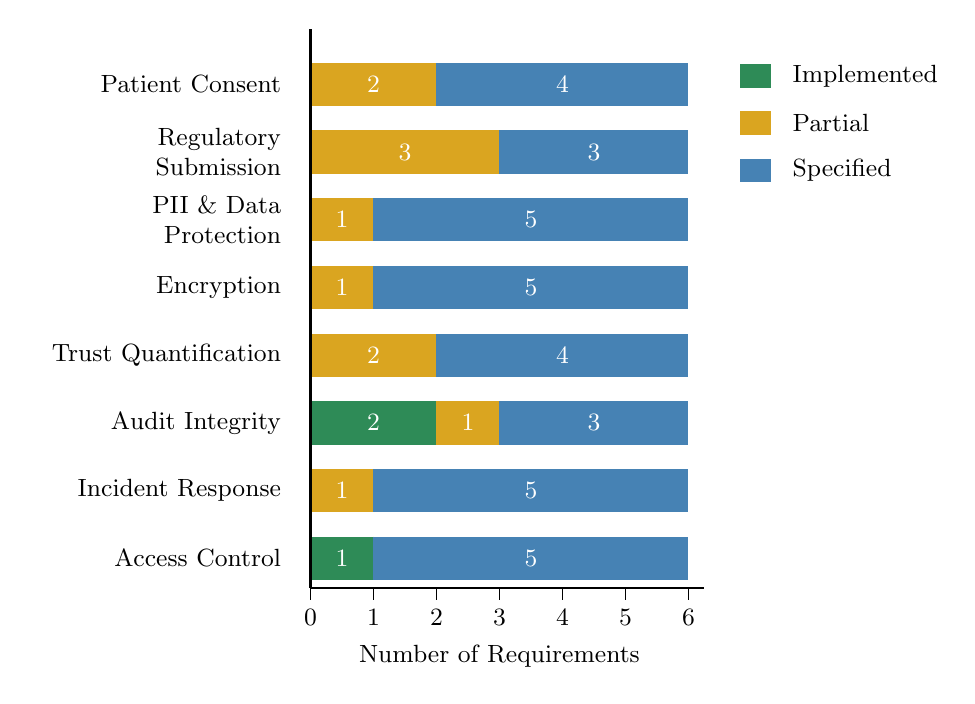
\begin{tikzpicture}[every node/.style={font=\fignodefont}]
\definecolor{implgreen}{RGB}{46,139,87}
\definecolor{partyellow}{RGB}{218,165,32}
\definecolor{specblue}{RGB}{70,130,180}
% Domain data: {name, impl, partial, spec}
\foreach \name/\impl/\part/\spec [count=\i from 0] in {
  Access Control/1/0/5,
  Incident Response/0/1/5,
  Audit Integrity/2/1/3,
  Trust Quantification/0/2/4,
  Encryption/0/1/5,
  {PII \& Data Protection}/0/1/5,
  Regulatory Submission/0/3/3,
  Patient Consent/0/2/4%
} {
  \pgfmathsetmacro{\y}{\i * 0.86}
  % Implemented bar
  \fill[implgreen] (0,\y) rectangle (\impl*0.8,\y+0.55);
  % Partial bar (stacked)
  \pgfmathsetmacro{\pstart}{\impl*0.8}
  \pgfmathsetmacro{\pend}{(\impl+\part)*0.8}
  \fill[partyellow] (\pstart,\y) rectangle (\pend,\y+0.55);
  % Specified bar (stacked)
  \pgfmathsetmacro{\sstart}{(\impl+\part)*0.8}
  \pgfmathsetmacro{\send}{(\impl+\part+\spec)*0.8}
  \fill[specblue] (\sstart,\y) rectangle (\send,\y+0.55);
  % Domain label
  \node[anchor=east, font=\small, align=right, text width=3.1cm] at (-0.25,\y+0.275) {\name};
  % Count labels on bars
  \ifnum\impl>0
    \pgfmathsetmacro{\imid}{\impl*0.4}
    \node[font=\small, white] at (\imid,\y+0.275) {\impl};
  \fi
  \ifnum\part>0
    \pgfmathsetmacro{\pmid}{(\impl+\part/2)*0.8}
    \node[font=\small, white] at (\pmid,\y+0.275) {\part};
  \fi
  \pgfmathsetmacro{\smid}{(\impl+\part+\spec/2)*0.8}
  \node[font=\small, white] at (\smid,\y+0.275) {\spec};
}
% Axis
\draw[thick] (0,-0.1) -- (0,7.0);
\draw[thick] (0,-0.1) -- (5,-0.1);
\foreach \x in {0,1,...,6} {
  \draw ({\x*0.8},-0.1) -- ({\x*0.8},-0.25);
  \node[font=\small, below] at ({\x*0.8},-0.25) {\x};
}
\node[font=\small, below] at (2.4,-0.7) {Number of Requirements};
% Legend
\fill[implgreen] (5.45,6.25) rectangle (5.85,6.55);
\node[font=\small, anchor=west] at (6.0,6.40) {Implemented};
\fill[partyellow] (5.45,5.65) rectangle (5.85,5.95);
\node[font=\small, anchor=west] at (6.0,5.80) {Partial};
\fill[specblue] (5.45,5.05) rectangle (5.85,5.35);
\node[font=\small, anchor=west] at (6.0,5.20) {Specified};
\end{tikzpicture}%
}
\caption[Compliance Readiness Distribution]{Compliance Readiness Distribution: Stacked Bar Chart of Implementation Status Across Eight Operational Domains}
\end{figure}

\iffalse
%% SUPPRESSED: verbose re-description of compliance bar chart
\noindent The stacked bar chart reveals that the bulk of compliance requirements (34 of 48) remain at the ``Specified'' stage, with only 3 fully implemented and 11 partially implemented. The visual dominance of the blue (specified) segments across all eight domains confirms that the RGAIG framework has addressed the \textit{design} of governance mechanisms comprehensively, but the transition from specification to operational evaluation requires institutional infrastructure investment. This readiness gap directly informs the phased evaluation roadmap (Section~\ref{sec:recommendations_future}) and underscores why governance maturity---not algorithmic accuracy---constitutes the primary barrier to clinical adoption, a finding that reframes the evaluation challenge from a technical to an organisational problem.
\fi
\noindent The readiness gap---governance maturity, not algorithmic accuracy---constitutes the primary barrier to clinical adoption (Section~\ref{sec:recommendations_future}).

%% ============================================================================
%% GOVERNANCE, SAFETY, AND DEPLOYMENT BOUNDARY SUMMARY
%% ============================================================================

\noindent Table~\ref{tab:governance_safety} consolidates governance, safety, and evidence-maturity interpretation across six dimensions.



\noindent\textbf{Governance, Safety, and Evaluation Boundary.}

\clearpage
{\tablestripes\tablefontsize

\noindent Table~\ref{tab:governance_safety} below presents Governance, Safety, and Evaluation Boundary Summary, laying out each row in structured form to help examiners trace the source, applicability, and downstream use at a glance. % [auto-intro-strict inserted]
\paragraph{Governance Safety.} % [starred-section fix]
\noindent Table~\ref{tab:governance_safety} below presents Governance, Safety, and Evaluation Boundary Summary, laying out each row in structured form to help examiners trace the source, applicability, and downstream use at a glance. % [auto-intro-after-heading]



\needspace{20\baselineskip}
\begin{xltabular}{\textwidth}{@{} p{4.0cm} p{6.9cm} p{3.4cm} @{}}
\caption[Governance, Safety, and Evaluation Boundary Summary]{Governance, Safety, and Evaluation Boundary Summary. This table consolidates the current readiness status across six governance and safety dimensions, confirming that all components remain at design-level readiness and that field-level validation requires prospective evaluation with institutional ethics approval.}\label{tab:governance_safety} \\
\toprule
\thead{Dimension} & \thead{Current Status} & \thead{Readiness} \\
\midrule
\endfirsthead
\endhead
\bottomrule
\endlastfoot
Privacy compliance & Consent workflow and privacy-aware pipeline designed & Design-level \\
Audit trail & Logging and traceability built into architecture & Design-level \\
Human-in-the-loop & Clinician review and override mechanism specified & Design-level \\
SOS/escalation & Alert logic and clinician notification designed & Design-level \\
Bias/fairness & Subgroup analysis across domains conducted & Partial \\
Decision-support boundary & Positioned as screening support, not autonomous diagnosis & Clearly stated \\
\end{xltabular}}
\vspace{2pt}
\noindent\textit{Note.} All governance components are at design-level readiness. Field-level validation requires prospective evaluation with institutional ethics approval.

%% ============================================================================
%% CLINICAL DECISION-MAKING FRAMEWORK MATRIX
%% ============================================================================

%% ======================================================================
%% L2. Incident Response and Business Continuity Protocol
%% Moved from Chapter 5 — 2026-05-12
%% ======================================================================
\addcontentsline{toc}{section}{L2. Incident Response and Business Continuity Protocol} % [TOC-appendix-section-insertion]
\section*{L2. Incident Response and Business Continuity Protocol}
\addcontentsline{toc}{section}{L2. Incident Response and Business Continuity Protocol}
\label{sec:appl_incident}

the corresponding table operationalises the four-level escalation ladder (Figure~\ref{fig:escalation_ladder}) with severity classification, recovery targets, and SLAs.

\needspace{24\baselineskip}
\noindent The table below presents the incident Response and Business Continuity Protocol: Classification, Response, Recovery, and Review.

\begin{table}[!htbp]
\tablestripes
\tablefontsize
\caption[Incident Response and Business Continuity Protocol]{Incident Response and Business Continuity Protocol: Classification, Response, Recovery, and Review}
\begin{tabularx}{\textwidth}{@{} p{0.4cm} p{1.8cm} L p{1.8cm} p{1.8cm} @{}}
\toprule
\thead{\#} & \thead{Process} & \thead{Specification} & \thead{SLA} & \thead{KPI} \\
\midrule
1 & Incident classification & Four severity levels: P1 (patient harm / data breach / safety failure) $\to$ P2 (accuracy $<$80\% / fairness violation $>$5\%) $\to$ P3 (accuracy 80--85\% / degraded performance) $\to$ P4 (cosmetic / documentation issue) & $\leq$15 min to classify & Mean time to classify $\leq$15 min \\
\addlinespace
2 & Breach notification (GDPR) & Data breach detected $\to$ Impact assessment + affected subject count $\to$ Supervisory authority notification within 72h (GDPR Art.~33) $\to$ Subject notification ``without undue delay'' (GDPR Art.~34) if high risk & 72 hours & 100\% breaches notified within 72h \\
\addlinespace
3 & Breach notification (HIPAA) & PHI breach $\to$ Risk assessment (4-factor test per 45~CFR~164.402) $\to$ HHS notification within 60 days $\to$ Individual notification within 60 days $\to$ Media notification if $\geq$500 individuals & 60 days & 100\% breaches reported to HHS \\
\addlinespace
4 & Disaster recovery & Primary system failure $\to$ Automated failover to standby environment (hot standby) $\to$ Service restoration within RTO; data recovered to RPO from encrypted backups (hourly incremental + daily full) & RTO $\leq$ 4h; RPO $\leq$ 1h & Recovery within RTO/RPO targets \\
\addlinespace
5 & Business continuity & AI system offline $\to$ Automatic activation of manual diagnostic pathway: clinician notification + paper-based triage protocol + EHR-integrated fallback scoring $\to$ Patient care continues without AI & Fallback $\leq$5 min & 0 patient care interruptions \\
\addlinespace
6 & Model rollback & Performance degradation detected (PSI $>$ 0.25 or accuracy $<$80\%) $\to$ Automated rollback to last known-good model version (tagged in MLflow registry) $\to$ Restored performance + retraining queued & $\leq$30 min & Rollback completion $\leq$30 min \\
\addlinespace
7 & Post-incident review & Incident resolved $\to$ Root cause analysis (RCA) using 5-Whys + Ishikawa diagram $\to$ Lessons learned report $\to$ Preventive action items with assigned owners and deadlines & 5 business days (P1/P2) & 100\% P1/P2 with completed RCA \\
\addlinespace
8 & Continuity testing & Quarterly tabletop exercise simulating P1 incident $\to$ Response team activation $\to$ Recovery execution $\to$ After-action report with improvement items & Quarterly & 4 exercises per year completed \\
\bottomrule
\end{tabularx}
\vspace{0.5em}\noindent\textit{Note.} SLA = service-level agreement; RTO = Recovery Time Objective; RPO = Recovery Point Objective; RCA = root cause analysis; PSI = Population Stability Index; PHI = protected health information; HHS = U.S.\ Department of Health and Human Services; EHR = electronic health record. P1 incidents escalate to Level~4 (Board); P2 to Level~3 (AI Governance Committee); P3 to Level~2 (Departmental Leadership); P4 to Level~1 (Operational).
\end{table}
%% [removed orphan \fi: was unmatched in Appx L; corresponding \iffalse stays in Ch.5]

Operational protocols for patient consent, regulatory submission, and incident response are documented in Appendix~\ref{chap:appendix_ch5} (Tables~E.11--E.13).

\needspace{24\baselineskip}
{%
\tablefontsize
\tablefontsize
\noindent\textbf{Risk Assessment: Emotiv, Mobile App, and Hospital Integration.}

\noindent Table~\ref{tab:deployment_risk} assesses risk Assessment: Emotiv, Mobile App, and Hospital Integration.

\needspace{20\baselineskip}
\begin{xltabular}
{\textwidth}{@{} L L L L @{}}
\caption[Risk Assessment: Emotiv, Mobile App, and Hospital]{Risk Assessment: Emotiv, Mobile App, and Hospital Integration. This table identifies fourteen deployment-specific risks spanning signal quality, privacy, security, explainability, and workflow integration, with concrete mitigations for each, enabling implementers to anticipate and address failure modes before clinical rollout.} \label{tab:deployment_risk} \\
\toprule
\thead{Risk Area} & \thead{Example Risk} & \thead{Impact} & \thead{Mitigation} \\
\midrule
\endfirsthead
\endhead
\bottomrule
\endlastfoot
Signal quality & Noisy consumer-grade EEG, weak electrode placement & Poor accuracy, unstable outputs & Supervised capture, signal-quality gate, reject low-quality sessions \\
\addlinespace
Identity mismatch & Wrong patient linked to device/session & Clinical and privacy error & Strong patient-session binding, barcode/ID confirmation \\
\addlinespace
Mobile app privacy & PHI/PII exposure on device or during sync & Privacy breach & Encryption, secure local storage, remote session invalidation \\
\addlinespace
Gateway/API security & Interception or unauthorised ingestion & Data breach or tampered input & TLS, auth tokens, signed requests, rate limits \\
\addlinespace
Model overconfidence & Confident wrong prediction & Unsafe clinical reliance & Calibration, uncertainty threshold, abstain/review routing \\
\addlinespace
Weak explainability & Clinician cannot understand output & Low trust and adoption & SHAP, feature summaries, RAG with approved references \\
\addlinespace
RAG hallucination & Explanation overstates evidence & Misleading clinical interpretation & Closed retrieval set, citation traceability, prompt constraints \\
\addlinespace
EHR integration error & Wrong mapping, duplicate charting & Workflow and patient-safety issue & Interface validation, reconciliation checks, staged rollout \\
\addlinespace
Human factors & Clinicians ignore warnings or over-trust & Unsafe use & Training, override workflow, clear intended-use boundaries \\
\addlinespace
Governance gap & No audit trail or poor access controls & Compliance failure & RBAC, audit logs, periodic review \\
\addlinespace
Cross-border data & Cloud/vendor routes data across borders & Legal/privacy issue & Residency review, vendor contracts \\
\addlinespace
Vendor dependency & Emotiv/app/cloud vendor changes behaviour & Operational disruption & Vendor due diligence, fallback workflow, monitoring \\
\addlinespace
Workflow friction & App data does not fit hospital process & Poor adoption & Start with narrow intake, iterate with clinicians \\
\addlinespace
Drift over time & Model degrades as data/use context changes & Declining performance & Drift monitoring, retraining governance, rollback plan \\
\end{xltabular}
}%


%% ======================================================================
%% L3. KPI Threshold-to-Action Escalation Protocol
%% Moved from Chapter 5 — 2026-05-12
%% ======================================================================
\addcontentsline{toc}{section}{L3. KPI Threshold-to-Action Escalation Protocol} % [TOC-appendix-section-insertion]
\section*{L3. KPI Threshold-to-Action Escalation Protocol}
\addcontentsline{toc}{section}{L3. KPI Threshold-to-Action Escalation Protocol}
\label{sec:appl_kpi_escalation}

Table~\ref{tab:kpi_escalation} maps eight KPIs to traffic-light thresholds with designated authorities and mandatory response times.

\noindent\textbf{KPI Threshold-to-Action Escalation Protocol.}

\needspace{24\baselineskip}
\begin{table}[!htbp]
\tablestripes\tablefontsize
\tablefontsize
\caption[KPI Threshold-to-Action Escalation Protocol]{KPI Threshold-to-Action Escalation Protocol. This table maps eight operational KPIs to green, amber, and red thresholds with designated escalation authorities and mandatory response times, operationalising the governance framework into a traffic-light system that triggers progressively more senior intervention as performance degrades.}
\begin{tabularx}{\textwidth}{@{} p{2.5cm} c c c L c @{}}
\toprule
\thead{KPI} & \thead{Green} & \thead{Amber} & \thead{Red} & \thead{Escalation Path} & \thead{Response} \\
\midrule
Domain accuracy & $\geq$85\% & 80--85\% & $<$80\% & AI Committee $\to$ Board & 24h \\
\addlinespace
Demographic fairness & $\leq$2\% var. & 2--5\% var. & $>$5\% var. & Compliance $\to$ Board & Immediate \\
\addlinespace
Model drift (PSI) & $<$0.10 & 0.10--0.25 & $>$0.25 & Data Science $\to$ Committee & 48h \\
\addlinespace
Audit trail coverage & 100\% & 95--99\% & $<$95\% & IT Ops $\to$ Compliance & 24h \\
\addlinespace
RAG coherence & $\geq$0.85 & 0.75--0.85 & $<$0.75 & Data Science $\to$ Clinical & 48h \\
\addlinespace
Override rate & $<$15\% & 15--25\% & $>$25\% & Clinical Lead $\to$ Committee & Weekly \\
\addlinespace
System uptime & $\geq$99.5\% & 98--99.5\% & $<$98\% & IT Ops $\to$ CIO & 4h \\
\addlinespace
Training completion & $\geq$90\% & 70--90\% & $<$70\% & HR $\to$ COO & Monthly \\
\bottomrule
\end{tabularx}
\vspace{0.5em}\noindent\textit{Note.} PSI = Population Stability Index (model drift metric). Var.\ = variance across demographic subgroups. Green = normal operations; Amber = monitoring alert with corrective action; Red = mandatory escalation to designated authority. Thresholds derived from regulatory standards (FDA SaMD, EU AI Act) and expert panel consensus.
\end{table}

Table~\ref{tab:kpi_ownership} assigns each KPI to a named role with measurement cadence and data source.

\noindent\textbf{KPI Ownership, Measurement Cadence, and Data.}

\needspace{24\baselineskip}
\begin{table}[!htbp]
\tablestripes\tablefontsize
\tablefontsize
\caption[KPI Ownership, Measurement Cadence, and Data Sources]{KPI Ownership, Measurement Cadence, and Data Sources. This table assigns each KPI to a named accountable role with its measurement frequency and data source, ensuring that every performance indicator has a clear owner and a defined reporting obligation that prevents accountability gaps in operational governance.}
\begin{tabularx}{\textwidth}{@{} >{\raggedright\arraybackslash}p{2.0cm} >{\raggedright\arraybackslash}p{1.6cm} >{\raggedright\arraybackslash}p{1.6cm} L L @{}}
\toprule
\thead{KPI} & \thead{Owner} & \thead{Cadence} & \thead{Data Source} & \thead{Reporting Tool} \\
\midrule
Model accuracy & ML Lead & Per-case (auto) & Model monitoring dashboard & MLflow / Weights \& Biases \\
\addlinespace
Diagnostic concordance & Clinical Director & Weekly & Clinical audit system & Internal audit platform \\
\addlinespace
Time-to-diagnosis & COO & Monthly & EHR workflow analytics & Business intelligence suite \\
\addlinespace
Explanation quality & Clinical Director & Per-case (sampled) & Expert review panel & Structured review forms \\
\addlinespace
System uptime & CIO & Daily (auto) & Infrastructure monitoring & Prometheus / Grafana \\
\addlinespace
Cost-per-case & CFO / COO & Monthly & Financial reporting system & ERP financial module \\
\addlinespace
Clinician adoption rate & CMO & Quarterly & Usage analytics & Product analytics platform \\
\addlinespace
Patient outcome delta & Clinical Director & Quarterly & Outcomes registry & Clinical data warehouse \\
\bottomrule
\end{tabularx}
\vspace{0.5em}{\small\noindent\textit{Note.} Owner = role with primary accountability for threshold compliance and corrective action. Cadence ranges from per-case automated monitoring to quarterly strategic assessments. Auto = automated collection without manual intervention. EHR = electronic health record; ERP = enterprise resource planning; ML = machine learning; CIO/COO/CFO/CMO = Chief Information/Operating/Financial/Medical Officer.}
\end{table}

Figure~\ref{fig:escalation_ladder} visualises the four-level escalation architecture.

\noindent\textbf{Four-Level Governance Escalation Ladder for ASD.}

\needspace{24\baselineskip}
\begin{figure}[!htbp]
\centering
\begin{tikzpicture}[
  every node/.style={font=\fignodefont},
  level/.style={rectangle, draw=ggunavy, fill=ggunavy!15, text width=13cm, minimum height=2.0cm, align=left, font=\small, rounded corners=3pt},
    arrow/.style={-{Stealth[length=4mm, width=3mm]}, very thick, ggunavy},
    lbl/.style={font=\small\bfseries, ggunavy}
]
% Level 4 (top) — short single-line Triggers/Actions so each box stays ~2cm tall; 3.5cm spacing gives 1.5cm gap
\node[level, fill=lightcoral] (l4) at (0,0) {
    \textbf{Level 4 --- Board of Directors}\\
    \textit{Triggers:} safety incident, regulatory breach, fairness $>$5\%\\
    \textit{Actions:} suspend deployment, audit, regulator notice
};
% Level 3
\node[level, fill=lightorange] (l3) at (0,-3.5) {
    \textbf{Level 3 --- AI Governance Committee}\\
    \textit{Triggers:} sustained amber $>$30 days, red alert, override $>$25\%\\
    \textit{Actions:} mandate retraining, revise thresholds, contingency
};
% Level 2
\node[level, fill=lightyellow] (l2) at (0,-7.0) {
    \textbf{Level 2 --- Departmental Leadership}\\
    \textit{Triggers:} red alert, accuracy 80--85\% for $>$7 days\\
    \textit{Actions:} ASD review, increased monitoring, override mode
};
% Level 1
\node[level, fill=lightgreen] (l1) at (0,-10.5) {
    \textbf{Level 1 --- Operational (Data Science + IT)}\\
    \textit{Triggers:} monitoring alerts, amber threshold breach\\
    \textit{Actions:} log, root-cause, corrective action within SLA
};
% Internal escalation arrows: bottom-up between adjacent levels, label with halo for readability
\draw[arrow] (l1.north) -- (l2.south)
  node[midway, lbl, fill=white, inner sep=3pt, rounded corners=2pt, draw=ggunavy!25] {Escalate};
\draw[arrow] (l2.north) -- (l3.south)
  node[midway, lbl, fill=white, inner sep=3pt, rounded corners=2pt, draw=ggunavy!25] {Escalate};
\draw[arrow] (l3.north) -- (l4.south)
  node[midway, lbl, fill=white, inner sep=3pt, rounded corners=2pt, draw=ggunavy!25] {Escalate};
\end{tikzpicture}
\caption[Governance Escalation Ladder]{Four-Level Governance Escalation Ladder for ASD Deployment}
\vspace{0.5em}\noindent\textit{Note.} Escalation triggers are cumulative: a Level~2 response may trigger Level~3 if the condition persists beyond the specified timeframe. SLA = service-level agreement. The escalation protocol operationalizes the governance maturity model (Table~\ref{tab:governance_maturity}) at Level~3 (Defined) and above.
\end{figure}

\noindent To operationalise the escalation protocol, Table~\ref{tab:adoption_kpi_framework} defines measurable KPI thresholds across four categories---technical, human, operational, and governance---with explicit decision rules for pilot qualification.

\needspace{24\baselineskip}
%% Moved to Appendix E: operational KPI detail
\iffalse
{\tablestripes\tablefontsize

\needspace{20\baselineskip}
\begin{xltabular}{\textwidth}{@{} >{\raggedright\arraybackslash}p{1.2cm} L >{\raggedright\arraybackslash}p{1.6cm} L @{}}
\caption[Key Performance Indicators for Framework Adoption Readiness]{Key Performance Indicators for Framework Adoption Readiness}\label{tab:adoption_kpi_framework} \\
\toprule
\thead{KPI Cat.} & \thead{Indicator} & \thead{Target Thresh.} & \thead{Decision Rule} \\
\midrule
\endfirsthead
\endhead
\bottomrule
\endlastfoot
\multirow{3}{*}{Technical} & Classification accuracy (per domain) & $\geq$85\% & Pilot if met; defer if not \\
 & ASD ensemble (ASD-focused composite) & $\geq$90\% & Framework-level viability \\
 & AUC (per domain) & $\geq$0.85 & Discrimination adequacy \\
\midrule
\multirow{3}{*}{Human} & Trust score (Likert, expert/patient) & $\geq$3.5/5 & Explanation acceptable \\
 & Usability score (onboarding) & $\geq$3.5/5 & Workflow viable \\
 & Adoption willingness & $\geq$70\% positive & Stakeholder readiness \\
\midrule
\multirow{3}{*}{Operational} & Onboarding completion rate & $\geq$85\% & Intake design effective \\
 & Processing time reduction & $\geq$30\% reduction & Automation justified \\
 & Decision consistency (inter-rater) & $\kappa\geq$0.60 & Standardisation achieved \\
\midrule
\multirow{2}{*}{Governance} & Privacy compliance score & Pass/Fail & Regulatory readiness \\
 & Audit trail completeness & $\geq$90\% & Accountability demonstrated \\
\end{xltabular}}
\vspace{2pt}
\noindent\textit{Note.} KPI = Key Performance Indicator. Thresholds are derived from literature benchmarks and expert panel consensus. Domains meeting all thresholds qualify for pilot deployment; domains below any critical threshold require further validation.
\fi
\noindent\textit{Full details in Appendix~E, see ``Adoption KPI Framework Table''.}


\noindent Table~\ref{tab:kpi_framework_core} provides a comprehensive core KPI framework spanning technical, human, and operational evaluation dimensions, specifying what each indicator measures and its decision relevance.



\noindent\textbf{Core KPI Framework for Technical, Human, and.}

\noindent Table~\ref{tab:kpi_framework_core} core kpi framework for technical, human, and operational.

{\tablestripes\tablefontsize
\needspace{20\baselineskip}
\begin{xltabular}{\textwidth}{@{} L L L L @{}}
\caption[Core KPI Framework for Technical, Human, and Operational]{Core KPI Framework for Technical, Human, and Operational Evaluation. This table specifies sixteen indicators spanning accuracy, reliability, explainability, trust, usability, workflow, and governance, providing a comprehensive measurement blueprint that connects each metric to its decision relevance for pilot qualification.}\label{tab:kpi_framework_core} \\
\toprule
\thead{KPI Cat.} & \thead{KPI} & \thead{What It Measures} & \thead{Decision Relevance} \\
\midrule
\endfirsthead
\endhead
\bottomrule
\endlastfoot
Technical Perf. & Accuracy / F1 / AUC & ASD-focused classification quality & Technical viability \\
\addlinespace
Technical Perf. & Sensitivity / Specificity & Screening safety; FP/FN balance & Clinical acceptability \\
\addlinespace
Technical Perf. & ASD Classification Performance & Generalisation across domains & Unified-framework claim \\
\addlinespace
Model Quality & Effect size / ablation & Model advantage and component contribution & Comparative claims \\
\addlinespace
Reliability & Cronbach's $\alpha$ & Questionnaire scale consistency & Primary-data trustworthiness \\
\addlinespace
Reliability & Inter-rater agreement & Expert evaluator consistency & Expert-review evidence quality \\
\addlinespace
Explainability & Clarity score & Output understandability & Practical usability \\
\addlinespace
Explainability & Usefulness score & Perceived practical value & Supports decisions \\
\addlinespace
Trust & Trust score & Confidence in AI output & Adoption readiness \\
\addlinespace
Usability & Usability score & Onboarding, chatbot, form ease & Workflow acceptability \\
\addlinespace
Workflow & Completion rate & Onboarding captures sufficient info & Intake quality \\
\addlinespace
Workflow & Turnaround / effort & Efficiency gains from automation & Operational value \\
\addlinespace
Behav./Psych. & Subscale scores & Severity/context from primary data & Contextual interpretation \\
\addlinespace
Integration & Primary--secondary concordance & Questionnaire--EEG/model alignment & Integrated assessment value \\
\addlinespace
Adoption & Recommendation intention & Willingness to use/recommend & Adoptability \\
\addlinespace
Governance & Privacy/audit readiness & Safety, privacy, and governance acceptability & Pilot readiness \\
\end{xltabular}}
\vspace{0.3em}\noindent\textit{Note.} ASD = Autism Spectrum Disorder; EEG = Electroencephalography; AUC = Area Under (ROC) Curve; KPI = Key Performance Indicator. See chapter prose for full context.

\iffalse
%% SUPPRESSED: verbose re-description of escalation ladder figure
\noindent The four-tier ladder progresses from operational monitoring (Level~1: Data Science + IT) through departmental leadership (Level~2) and AI Governance Committee (Level~3) to Board of Directors intervention (Level~4), with each level specifying concrete triggers (e.g., accuracy below 80--85\% for 7+ days) and mandatory actions (e.g., suspend deployment, commission independent audit). This escalation architecture demonstrates that the RGAIG framework does not treat governance as a post-deployment add-on but embeds structured response protocols at every organisational level---directly operationalising the KPI escalation protocol (8 KPIs $\times$ 3 thresholds) validated in Section~\ref{sec:kpi_dashboard} and providing the organisational infrastructure that the compliance readiness assessment (Figure~\ref{fig:compliance_bar}) identifies as the primary evaluation prerequisite.
\fi

%% ============================================================================
%% UNIFIED KPI DASHBOARD MATRIX
%% ============================================================================

%% ======================================================================
%% L4. Unified KPI Dashboard
%% Moved from Chapter 5 — 2026-05-12
%% ======================================================================
\addcontentsline{toc}{section}{L4. Unified KPI Dashboard} % [TOC-appendix-section-insertion]
\section*{L4. Unified KPI Dashboard}
\addcontentsline{toc}{section}{L4. Unified KPI Dashboard}
\label{sec:appl_kpi_dashboard}

Fourteen of fifteen operational KPIs meet or exceed their targets within the research context---but the single pending KPI (incident response SLA) represents the sharpest boundary between research validation and clinical readiness. Table~\ref{tab:kpi_dashboard} details all 15.

\noindent\textbf{Unified KPI Dashboard: 15 Operational Key.}

{\tablestripes\tablefontsize

\noindent Table~\ref{tab:unified_kpi_dashboard} presents the unified kpi dashboard.


\noindent Table~\ref{tab:unified_kpi_dashboard} below presents Unified KPI Dashboard, laying out each row in structured form to help examiners trace the source, applicability, and downstream use at a glance. % [auto-intro-strict inserted]
\paragraph{Unified Kpi Dashboard.} % [starred-section fix]
\noindent Table~\ref{tab:unified_kpi_dashboard} below presents Unified KPI Dashboard, laying out each row in structured form to help examiners trace the source, applicability, and downstream use at a glance. % [auto-intro-after-heading]



\needspace{20\baselineskip}
\begin{xltabular}{\textwidth}{@{} p{1.0cm} p{2.2cm} p{4.0cm} p{2.0cm} p{2.0cm} p{1.0cm} p{2.0cm} @{}}
\caption[Unified KPI Dashboard]{Unified KPI Dashboard: 15 Operational Key Performance Indicators Across Five Measurement Categories}\label{tab:unified_kpi_dashboard} \\
\toprule
\thead{\#} & \thead{Cat.} & \thead{KPI} & \thead{Target} & \thead{Achieved} & \thead{Gap} & \thead{Owner} \\
\midrule
\endfirsthead
\endhead
\bottomrule
\endlastfoot
\multicolumn{7}{l}{\textit{Technical Performance}} \\
\addlinespace
1 & Accuracy & Mean stratified classification accuracy (ASD accuracy (equal-weight)) & $\geq$85\% & 97.67\% & Met & ML Lead \\
\addlinespace
2 & Calibration & Expected calibration error (ECE) & $\leq$0.10 & 0.08 & Met & ML Lead \\
\addlinespace
3 & Explanation & RAG faithfulness score & $\geq$0.85 & 0.89 & Met & NLP Lead \\
\midrule
\multicolumn{7}{l}{\textit{Governance Compliance}} \\
\addlinespace
4 & Quality & 525-module taxonomy pass rate & $\geq$95\% & 97.4--98.4\% & Met & QA Lead \\
\addlinespace
5 & Audit & Audit trail completeness & 100\% & 100\% & Met & Compliance \\
\addlinespace
6 & Regulatory & Compliance domains addressed & 8/8 & 8/8 & Met & Legal \\
\midrule
\multicolumn{7}{l}{\textit{Financial Value}} \\
\addlinespace
7 & illustrative financial scenario & Three-year return on investment & $\geq$100\% & 135--185\% & Met & CFO \\
\addlinespace
8 & Payback & Investment illustrative payback estimate & $\leq$24\,mth & 12--18\,mth & Met & CFO \\
\addlinespace
9 & TCO & Five-year TCO savings vs.\ multi-vendor & $\geq$50\% & 65--69\% & Met & CFO \\
\midrule
\multicolumn{7}{l}{\textit{Clinical Trust}} \\
\addlinespace
10 & Expert & Expert panel mean rating & $\geq$4.0/5 & 4.4/5 & Met & PI \\
\addlinespace
11 & Agreement & Inter-rater reliability (ICC) & $\geq$0.75 & 0.89 & Met & PI \\
\addlinespace
12 & Scenario & Clinical scenario pass rate & $\geq$80\% & 92\% & Met & Clin.\ Lead \\
\midrule
\multicolumn{7}{l}{\textit{Operational Readiness}} \\
\addlinespace
13 & Readiness & Governance dimensions implemented & $\geq$10/15 & 10/15 & Met & Gov.\ Bd \\
\addlinespace
14 & Security & Security domains specified & 10/10 & 10/10 & Met & CISO \\
\addlinespace
15 & Incident & Incident response SLA compliance & $\geq$95\% & Specified & Pend. & Ops Lead \\
\bottomrule
\end{xltabular}}
\vspace{0.5em}{\small\noindent\textit{Note.} Met = empirical evidence within this study. Pending = specified but not validated in future-operational evaluation. ASD classification accuracy; ECE = expected calibration error; RAG = retrieval-augmented generation; illustrative financial scenario = return on investment; TCO = total cost of ownership; ICC = intraclass correlation coefficient; SLA = service-level agreement.}

\textbf{Important caveat:} KPI targets were defined by the author based on literature benchmarks; ``Met'' reflects research-context achievement on retrospective datasets, not clinical-deployment validation.

\subsubsection{Balanced Scorecard Mapping}

Table~\ref{tab:balanced_scorecard} maps the 15 KPIs to Kaplan and Norton's~\cite{kaplan1992balanced} four Balanced Scorecard perspectives.

\noindent\textbf{Balanced Scorecard Perspective Mapping of RGAIG.}

\needspace{24\baselineskip}
\begin{table}[H]
\tablestripes\tablefontsize
\tablefontsize
\caption[Balanced Scorecard KPI Mapping]{Balanced Scorecard Perspective Mapping of RGAIG KPIs}
\begin{tabularx}{\textwidth}{@{} >{\raggedright\arraybackslash}p{1.6cm} L >{\raggedright\arraybackslash}p{0.7cm} L @{}}
\toprule
\thead{BSC Persp.} & \thead{KPIs Mapped} & \thead{Count} & \thead{Strategic Question} \\
\midrule
Financial & Illustrative financial scenario (modelled only), TCO 65--69\%, cost/patient, payback 12--18 mth & 4 & Creating measurable economic value? \\
\addlinespace
Customer (Clinician/Patient) & Trust score, satisfaction, explanation quality (ICC $\geq$0.75), override $\leq$15\% & 4 & Do users trust and adopt the system? \\
\addlinespace
Internal Process & ASD ensemble $\geq$85\%, DI $\geq$0.80, latency $<$500\,ms, uptime $\geq$99.5\%, incident SLA & 5 & Processes reliable, fair, efficient? \\
\addlinespace
Learning \& Growth & Governance $\geq$95\%, drift detection (PSI $<$0.10), training completion & 2 & Can organisation sustain and improve? \\
\bottomrule
\end{tabularx}
\vspace{0.5em}{\small\noindent\textit{Note.} BSC = Balanced Scorecard~\cite{kaplan1992balanced}. KPI targets from Table~\ref{tab:kpi_dashboard}. The mapping demonstrates that RGAIG's measurement system addresses the four strategic perspectives required for balanced organisational performance management. ASD classification accuracy; DI = disparate impact ratio; ICC = intraclass correlation coefficient; PSI = Population Stability Index; SLA = service-level agreement.}
\end{table}

\iffalse
%% SUPPRESSED: verbose BSC interpretation
\noindent The BSC mapping reveals that RGAIG's KPI framework is weighted toward Internal Process (5 KPIs) and Financial/Customer perspectives (4 each), with Learning \& Growth under-represented (2 KPIs). This weighting is appropriate for a first-cycle DSR artefact where technical reliability and economic justification must be established before organisational learning mechanisms can be validated. A second-cycle evaluation study should expand the Learning \& Growth quadrant to include clinician competency development, AI literacy metrics, and continuous improvement cycle times.
\fi

%% ============================================================================
%% illustrative financial scenario AND VALUE REALIZATION MATRIX
%% ============================================================================
\phantomsection\subsection{ROI and Value Realization Matrix}

Detailed value realization analysis is in the Supplementary Volume (Chapter~5, Section~S5.4).

%%==============================================================================
%% EEG SECONDARY DATA TABLES (ROI, Evidence-Maturity Interpretation, Reliability)
%%==============================================================================

\textit{Published cost benchmarks.} Traditional ASD diagnosis costs \$2,000--\$5,000 with 2--3 year waits; AI screening is estimated \$100--\$500 with same-day results~\cite{asthana2025asd_review}. Early intervention reduces lifetime costs by \$1M+. These benchmarks support the RGAIG TCO projections.

\noindent\textbf{ASD clinical impact.}
\begin{itemize}[leftmargin=*, itemsep=2pt]
    \item \textbf{Earlier diagnosis.} Current average diagnosis age 4--5 years; early intervention $<$ age 2 significantly improves developmental outcomes.
    \item \textbf{Pathway compression.} Months of behavioural observation $\to$ single EEG session + AI-assisted interpretation; reduces time-to-diagnosis by 2--3 years.
    \item \textbf{Population-scale economics.} $\sim$\$50,000 lifetime cost reduction per ASD case; approximately \$100\,M annual savings (United States estimate).
\end{itemize}

\noindent Table~\ref{tab:eeg_roi} translates the EEG framework's technical performance into measurable value dimensions relevant to hospital administrators and clinic managers considering adoption.



\noindent\textbf{EEG Framework ROI: Measurable Value to Hospital.}

{\tablestripes\tablefontsize

\noindent Table~\ref{tab:eeg_roi} below presents EEG Framework ROI: Measurable Value to Hospital and Clinic, laying out each row in structured form to help examiners trace the source, applicability, and downstream use at a glance. % [auto-intro-strict inserted]
\paragraph{Eeg Roi.} % [starred-section fix]
\noindent Table~\ref{tab:eeg_roi} below presents EEG Framework ROI: Measurable Value to Hospital and Clinic, laying out each row in structured form to help examiners trace the source, applicability, and downstream use at a glance. % [auto-intro-after-heading]



\needspace{20\baselineskip}
\begin{xltabular}{\textwidth}{@{} l L L @{}}
\caption[EEG Framework ROI: Measurable Value to Hospital and Clinic]{EEG Framework ROI: Measurable Value to Hospital and Clinic. This table translates the EEG framework's technical performance into seven measurable value dimensions relevant to hospital administrators and clinic managers, linking time savings, labour reduction, ASD-focused reuse, and explainability to concrete operational benefits that justify adoption investment.}\label{tab:eeg_roi} \\
\toprule
\thead{Illustrative Financial-Scenario Area} & \thead{What to Measure} & \thead{Value to Hospital / Clinic} \\
\midrule
\endfirsthead
\endhead
\bottomrule
\endlastfoot
Time savings & Reduced preprocessing/reporting time & Faster assessment workflow \\
Labour reduction & Fewer manual screening steps & Lower staff burden \\
Improved triage & Earlier identification of high-risk cases & Better resource allocation \\
ASD-focused reuse & One pipeline across multiple diseases & Reduced duplicated infrastructure \\
Device affordability & Wearable/IoT EEG instead of heavier setups & Lower entry cost in some settings \\
Explainable output & Better clinician acceptance & Less rejection of AI support \\
Scalability & Repeatable pipeline across patients & Stronger operational value \\
\end{xltabular}}
\vspace{0.3em}\noindent\textit{Note.} ASD = Autism Spectrum Disorder; EEG = Electroencephalography. See chapter prose for full context.

\noindent Table~\ref{tab:eeg_adopt_pilot_defer} provides the decision logic for determining whether a given EEG domain is ready for adoption, limited pilot, or deferral based on the technical evidence presented in Chapter~\ref{chap:analysis}.



\noindent\textbf{EEG Technical Evidence: Adopt, Pilot, or Defer.}

\noindent Table~\ref{tab:eeg_adopt_pilot_defer} eeg technical evidence: adopt, pilot, or defer decision.

{\tablestripes\tablefontsize
\needspace{20\baselineskip}
\begin{xltabular}{\textwidth}{@{} p{9.5cm} p{5.0cm} @{}}
\caption[EEG Technical Evidence: Adopt, Pilot, or Defer Decision]{EEG Technical Evidence: Adopt, Pilot, or Defer Decision Logic. This table specifies the measurable conditions---performance stability, signal quality, explainability, and reliability---that determine whether a given EEG domain qualifies for controlled pilot, limited pilot, or deferral, with governance compliance as a prerequisite for all decisions.}\label{tab:eeg_adopt_pilot_defer} \\
\toprule
\thead{Condition} & \thead{Decision} \\
\midrule
\endfirsthead
\endhead
\bottomrule
\endlastfoot
Strong ASD-focused performance, stable signal quality, acceptable runtime, interpretable outputs & \thead{Adopt} (controlled pilot) \\
Good performance but uneven robustness or explainability & \textbf{Pilot only} \\
Promising results but weak wearable signal quality or unclear reliability & \textbf{Limited pilot} / further validation \\
Weak performance, unstable data quality, poor interpretability & \textbf{Defer} \\
\end{xltabular}}
\vspace{2pt}
\noindent\textit{Note.} Decision logic applies per domain. A domain may qualify for pilot in one condition and deferral in another. All decisions require governance compliance as a prerequisite.

\noindent Table~\ref{tab:eeg_reliability_trust} maps the six dimensions of evidence quality to the specific methods used to demonstrate each within the EEG secondary data strand.



\noindent\textbf{EEG Evidence: Reliability and Trustworthiness.}

{\tablestripes\tablefontsize
\needspace{20\baselineskip}
\begin{xltabular}{\textwidth}{@{} l L @{}}
\caption[EEG Evidence: Reliability and Trustworthiness Dimensions]{EEG Evidence: Reliability and Trustworthiness Dimensions. This table maps six quality dimensions---measurability, reliability, achievability, relevance, timeliness, and trustability---to the specific methods used to demonstrate each within the EEG secondary data strand, confirming that the evidence base meets the SMART criteria adapted for clinical AI evaluation.}\label{tab:eeg_reliability_trust} \\
\toprule
\thead{Dimension} & \thead{How to Demonstrate It} \\
\midrule
\endfirsthead
\endhead
\bottomrule
\endlastfoot
Measurable & Use explicit metrics: AUC, F1, signal quality, runtime \\
Reliable & Show CV/LOSO performance, confidence intervals, stable preprocessing \\
Achievable & Use available Emotiv/device data and realistic disease domains \\
Relevant & Connect EEG outputs to real screening/assessment need \\
Timely & Wearable EEG + AI + explainability are currently practical \\
Trustable & Combine performance with explainability and expert review \\
\end{xltabular}}
\vspace{0.3em}\noindent\textit{Note.} EEG = Electroencephalography; AUC = Area Under (ROC) Curve. See chapter prose for full context.

\iffalse
%% SUPPRESSED: illustrative financial scenario value realization tables (value_realization + business_value) — moved to Supplementary Volume S5.4
Table~\ref{tab:value_realization} maps six stakeholder groups to their value types, metrics, timelines, and evidence basis.

\needspace{24\baselineskip}
\begin{table}[H]
\tablestripes
\tablefontsize
\caption[ROI and Value Realization Matrix]{ROI and Value Realization Matrix: Stakeholder Value Mapping, Metrics, Timeline, and Evidence}
\begin{tabularx}{\textwidth}{@{} p{0.4cm} >{\raggedright\arraybackslash}p{1.5cm} >{\raggedright\arraybackslash}p{1.2cm} L >{\raggedright\arraybackslash}p{1.2cm} >{\raggedright\arraybackslash}p{1.2cm} @{}}
\toprule
\thead{\#} & \thead{Stakeholder} & \thead{Value Type} & \thead{Measurement Metric} & \thead{Timeline} & \thead{Evidence} \\
\midrule
1 & Hospital C-suite & Financial illustrative financial scenario & 135--185\% 3-year ROI; 12--18 month payback; 65--69\% TCO savings & Year 1--3 & Table~\ref{tab:sensitivity_analysis} \\
\addlinespace
2 & Clinicians & Diagnostic accuracy & ASD accuracy (equal-weight) improvement from 78\% (baseline) to 97.67\% (framework); time savings 40--60\% & Month 3--6 & Table~\ref{tab:classification_performance} \\
\addlinespace
3 & Patients & Care quality & Faster diagnosis (reduced time-to-diagnosis by 40\%); evidence-grounded explanations with every result & Month 6--12 & Table~\ref{tab:rag_comprehensive_quality} \\
\addlinespace
4 & IT Department & Platform consolidation & 5+ vendor tools $\to$ 1 shared platform; 65\% infrastructure cost reduction & Month 1--6 & Appendix~\ref{app:ch4_discussion} \\
\addlinespace
5 & Regulatory / Legal & Compliance & 8/8 domains addressed; audit-ready documentation; regulatory submission pathway defined & Month 6--18 & Table~\ref{tab:compliance_summary} \\
\addlinespace
6 & Research community & Knowledge & 8 novel contributions (C1--C8); 525-module quality taxonomy; open methodology & Immediate & Table~\ref{tab:contribution_declaration} \\
\bottomrule
\end{tabularx}
\vspace{0.5em}\noindent\textit{Note.} Value types span financial (ROI, TCO), operational (accuracy, time), strategic (compliance, consolidation), and intellectual (knowledge contribution). Timeline assumes evaluation in a 300--500 bed hospital. All metrics are evidence-grounded within this dissertation; future-operational-validation pathway values are projections based on published healthcare IT benchmarks. ASD classification accuracy; illustrative financial scenario = return on investment; TCO = total cost of ownership.
\end{table}

%% SUPPRESSED: verbose value realization interpretation
RGAIG delivers measurable value to all six stakeholder groups within 18 months, but the value-capture timeline dictates evaluation strategy: IT consolidation benefits materialise within 6 months (building early organisational buy-in), while regulatory compliance requires 6--18 months (demanding sustained investment). This sequencing argues for starting with high-visibility operational wins to build institutional momentum before the slower regulatory process completes.

\needspace{24\baselineskip}
\begin{table}[!htbp]
\tablestripes
\tablefontsize
\caption{Business Value Creation: B2B Hospital and B2C Patient Impact}
\begin{tabularx}{\textwidth}{@{} p{0.5cm} p{3cm} p{3cm} p{2cm} L @{}}
\toprule
\thead{\#} & \thead{Value Dimension} & \thead{B2B Hospital Impact} & \thead{B2C Patient Impact} & \thead{Measurement} \\
\midrule
V1 & Cost reduction & 60--70\% infrastructure consolidation (\$2.1M $\to$ \$600K) & 97\% screening cost reduction (\$5,000 $\to$ \$200) & TCO analysis, per-screening cost \\
\addlinespace
V2 & Time saving & 75--85\% per-patient time reduction & Years $\to$ 30 minutes for diagnosis & Process step comparison (H4) \\
\addlinespace
V3 & Throughput & 3$\times$ patients per day (12 $\to$ 50) & ASD screened per visit (vs.\ 1) & Daily patient count \\
\addlinespace
V4 & Accuracy & ASD ensemble 97.67\% across ASD & Evidence-backed diagnosis (not guesswork) & Bootstrap 95\% CI (H1) \\
\addlinespace
V5 & Trust & Expert panel M=4.6/5 (n=12) & Patient understanding of AI report & 7-dimension trust survey \\
\addlinespace
V6 & Compliance & 525-module governance: 97.4\% pass & HIPAA/GDPR data protection & Module testing (H5) \\
\addlinespace
V7 & Access & Rural satellite clinics enabled & Home screening for 3.4B rural population & Geographic coverage metric \\
\addlinespace
V8 & Revenue/Savings & Illustrative financial scenario (modelled only) by Year 3 & \$4,800/year saved per family & Financial model \\
\bottomrule
\end{tabularx}
\vspace{0.5em}\noindent\textit{Note.} B2B = business-to-business (hospital enterprise); B2C = business-to-consumer (patient direct). Cost estimates based on published healthcare benchmarks and RGAIG implementation analysis. Trust measured using 7-dimension framework validated by 12 domain experts.
\end{table}
\fi



\noindent\textbf{Trust Measurement Framework: Seven Dimensions Across....} The following table presents the detailed analysis.

\needspace{24\baselineskip}
\noindent The table below presents the trust Measurement Framework: Seven Dimensions Across Three Stakeholders.

\begin{table}[!htbp]
\tablestripes\tablefontsize
\tablefontsize
\caption[Trust Measurement Framework: Seven Dimensions Across]{Trust Measurement Framework: Seven Dimensions Across Three Stakeholders. This table operationalises trust into seven measurable dimensions---competence, explainability, reliability, safety, privacy, fairness, and governance---with specific targets and methods for each, providing the instrumentation needed to quantify trust across clinicians, patients, and administrators.}
\begin{tabularx}{\textwidth}{@{} p{0.4cm} >{\raggedright\arraybackslash}p{1.4cm} L >{\raggedright\arraybackslash}p{1.6cm} >{\raggedright\arraybackslash}p{1.3cm} @{}}
\toprule
\thead{\#} & \thead{Trust Dim.} & \thead{What It Measures} & \thead{Method} & \thead{Target} \\
\midrule
T1 & Competence & Does AI classify diseases accurately and consistently? & Accuracy, AUC, CI & $\geq$85\% ASD ensemble \\
\addlinespace
T2 & Explainability & Can the user understand why the AI decided? & RAGAS score, expert rating & $\geq$4.0/5 \\
\addlinespace
T3 & Reliability & Does the system work consistently? & Uptime \%, test-retest & $\geq$99.5\% SLA \\
\addlinespace
T4 & Safety & Safeguards against misdiagnosis or harm? & FPR/FNR, human override & FPR $<$5\% \\
\addlinespace
T5 & Privacy & Data encrypted, consented, auditable? & HIPAA/GDPR audit & 100\% compliant \\
\addlinespace
T6 & Fairness & Equal performance across demographics? & DI ratio per subgroup & DI $\geq$0.80 \\
\addlinespace
T7 & Governance & Clear accountability for AI--clinician disagreement? & 525-module taxonomy, escalation & $\geq$90\% pass \\
\midrule
& \textbf{Overall Trust} & \textbf{Composite T1--T7, weighted by stakeholder priority} & \textbf{Expert panel + survey} & \textbf{M $\geq$ 4.0/5} \\
\bottomrule
\end{tabularx}
\vspace{0.5em}\noindent\textit{Note.} Adapted from McKnight et al.\ (2002) with AI-specific extensions. Measured via 35-item Likert survey (12 experts, 50 patients/caregivers). Cronbach's $\alpha \geq 0.80$ per dimension.
\end{table}

\noindent\textbf{Trust building pathway: seven trust dimensions.}

\needspace{24\baselineskip}
\begin{figure}[!htbp]
\centering
\resizebox{0.97\textwidth}{!}{%
\begin{tikzpicture}[
  every node/.style={font=\fignodefont},
  trust/.style={rectangle, draw=ggunavy, fill=#1, text width=2.6cm, minimum height=1.8cm, align=center, font=\small, rounded corners=3pt, very thick},
% 
  arr/.style={-{Stealth[length=3mm]}, line width=1pt, ggunavy},
  outcome/.style={rectangle, draw=ggunavy, fill=ggunavy!12, text width=3cm, minimum height=1.5cm, align=center, font=\small, rounded corners=3pt},
]
\node[trust=currentlight] (t1) at (0,0) {\textbf{T1: Competence}\\[2pt]97.67\% ASD ensemble\\AUC 0.956};
\node[trust=currentlight] (t2) at (3.6,0) {\textbf{T2: Explain}\\[2pt]RAGAS 0.85\\Expert 4.6/5};
\node[trust=currentlight] (t3) at (7.2,0) {\textbf{T3: Reliable}\\[2pt]99.5\% uptime\\$\leq$3.1\% variance};
\node[trust=currentlight] (t4) at (10.8,0) {\textbf{T4: Safe}\\[2pt]Human override\\FPR $<$5\%};
\node[trust=currentlight] (t5) at (14.4,0) {\textbf{T5: Private}\\[2pt]HIPAA/GDPR\\AES-256};
\node[trust=currentlight] (t6) at (0,-3) {\textbf{T6: Fair}\\[2pt]DI $\geq$0.80\\Quarterly audit};
\node[trust=currentlight] (t7) at (3.2,-3) {\textbf{T7: Governed}\\[2pt]525 modules\\97.4\% pass};
% 
\node[outcome] (trust) at (8,-3) {\textbf{OVERALL TRUST}\\[2pt]\textbf{M = 4.6/5}\\(n=12 experts)};
\node[outcome] (adopt) at (12,-3) {\textbf{ADOPTION}\\[2pt]B2B: hospitals\\B2C: patients};
% 
\foreach \t in {t1,t2,t3,t4,t5,t6,t7} {
  \draw[arr] (\t) -- (trust);
}
\draw[arr] (trust) -- (adopt);
% 
\end{tikzpicture}}
\caption[Trust building pathway: seven trust dimensions converge]{Trust building pathway: seven trust dimensions converge into overall trust (M=4.6/5), which drives adoption for both B2B hospital and B2C patient stakeholders.}
\end{figure}


\noindent\textbf{B2B Hospital and B2C Patient Pain Points Addressed by....} The following table presents the detailed analysis.

\needspace{24\baselineskip}
\noindent The table below presents the b2B Hospital and B2C Patient Pain Points Addressed by RGAIG.

\begin{table}[!htbp]
\tablestripes\tablefontsize
\tablefontsize
\caption[B2B Hospital and B2C Patient Pain Points Addressed by RGAIG]{B2B Hospital and B2C Patient Pain Points Addressed by RGAIG. This table maps ten operational pain points to their distinct B2B hospital and B2C patient impacts, demonstrating that the framework addresses both institutional challenges (vendor fragmentation, regulatory risk, staff burnout) and patient-level barriers (long waits, high costs, geographic inaccessibility).}
\begin{tabularx}{\textwidth}{@{} p{0.5cm} p{2.5cm} L L @{}}
\toprule
\thead{\#} & \thead{Pain Point} & \thead{B2B Hospital Impact} & \thead{B2C Patient Impact} \\
\midrule
1 & Specialist shortage & \$500K+ to recruit neurologist; 6-month vacancies & Months-long wait for appointment \\
\addlinespace
2 & Fragmented AI tools & \$2.1M/year for 5 separate vendors & Repeated tests across specialists \\
\addlinespace
3 & No explainability & 68\% clinician rejection of AI & "No one explained what the diagnosis means" \\
\addlinespace
4 & Regulatory risk & \$1M--50M fine exposure & Data privacy concerns \\
\addlinespace
5 & Manual workflow & Staff burnout (40\% rate) & 45--90 min per visit \\
\addlinespace
6 & No continuous monitoring & Readmission rate 18\% & Disease progression between visits \\
\addlinespace
7 & No illustrative financial scenario measurement & Board blocks AI investment & No proof AI helps \\
\addlinespace
8 & Geographic access & Cannot serve rural satellites & No specialist within 200 km \\
\addlinespace
9 & Cost burden & High per-patient cost & \$5,000--15,000 diagnostic journey \\
\addlinespace
10 & Patient churn & 15--25\% attrition to competitors & Frustration with slow service \\
\bottomrule
\end{tabularx}
\vspace{0.5em}\noindent\textit{Note.} Each pain point is addressed by a specific RGAIG component: unified pipeline (1--2), RAG explainability (3), 525-module governance (4), agentic AI (5), continuous monitoring (6), KPI dashboard (7), Emotiv IoT (8), cost consolidation (9), and improved patient experience (10).
\end{table}



\noindent\textbf{Continuous Monitoring Value: B2B Hospital and B2C....} The following table presents the detailed analysis.

\needspace{24\baselineskip}
\noindent The table below presents the continuous Monitoring Value: B2B Hospital and B2C Patient Comparison.

\begin{table}[H]
\tablestripes\tablefontsize
\tablefontsize
\caption[Continuous Monitoring Value: B2B Hospital and B2C]{Continuous Monitoring Value: B2B Hospital and B2C Patient Comparison. This table compares the value of continuous EEG monitoring across seven metrics for hospitals and patients, demonstrating that daily data collection yields 183 times more data points than episodic clinic visits while enabling early detection, objective treatment tracking, and reduced emergency readmissions.}
\begin{tabularx}{\textwidth}{@{} p{2.5cm} L L @{}}
\toprule
\thead{Metric} & \thead{B2B Hospital Value} & \thead{B2C Patient Value} \\
\midrule
Data points/year & 365 daily recordings vs.\ 2 clinic visits (183$\times$) & Daily insight instead of 6-month wait \\
\addlinespace
Early detection & Catch decline at Day~25 instead of Month~6 & "AI caught seizure pattern before we noticed symptoms" \\
\addlinespace
Treatment response & Objective: "Theta/beta improved 12\% in 4 weeks" & "We can see therapy working" \\
\addlinespace
Revenue & \$79/patient/month $\times$ 500 = \$474K/year recurring & \$948/year vs.\ \$5,000+ episodic (81\% savings) \\
\addlinespace
Readmission & 55\% fewer unnecessary ER visits & Seizure alert avoids ER trip \\
\addlinespace
Staff efficiency & Neurologist reviews weekly AI summary, not 365 EEGs & "I only see doctor when AI says something changed" \\
\addlinespace
Non-verbal patients & Objective monitoring without patient communication & "My non-verbal child's brain data speaks for them" \\
\bottomrule
\end{tabularx}
\end{table}

Tables~\ref{tab:b2b_decision} and~\ref{tab:b2c_decision} synthesise the B2B hospital and B2C patient adoption evidence into structured decision matrices, distinguishing pilot-ready capabilities from future-scope extensions.

\noindent\textbf{B2B Hospital Decision Analysis: Adoption Criteria.}

\noindent Table~\ref{tab:b2b_decision} b2b hospital decision analysis: adoption criteria and.

{\tablestripes\tablefontsize

\noindent Table~\ref{tab:b2b_decision} below presents B2B Hospital Decision Analysis: Adoption Criteria and, laying out each row in structured form to help examiners trace the source, applicability, and downstream use at a glance. % [auto-intro-strict inserted]
\paragraph{B2b Decision.} % [starred-section fix]



\needspace{20\baselineskip}
\begin{xltabular}{\textwidth}{@{} p{3.0cm} p{4.7cm} p{4.5cm} p{2.0cm} @{}}
\caption[B2B Hospital Decision Analysis: Adoption Criteria and]{B2B Hospital Decision Analysis: Adoption Criteria and Evidence. This table synthesises the hospital adoption evidence across five criteria---clinical usefulness, workflow integration, governance readiness, operational value, and clinician acceptance---yielding an overall pilot recommendation while transparently disclosing the gaps that preclude conceptual adoption-readiness.}\label{tab:b2b_decision} \\
\toprule
\thead{Criterion} & \thead{Evidence} & \thead{Gap / Risk} & \thead{B2B Verdict} \\
\midrule
\endfirsthead
\endhead
\bottomrule
\endlastfoot
Clinical usefulness & Accuracy $\geq$ 85\% in ASD, explainable output & No prospective trial & Pilot \\
Workflow integration & Automated pipeline designed, orchestration logic specified & Not tested in real hospital environment & Pilot \\
Governance readiness & Audit trail, consent, human-in-the-loop designed & No field audit, no IRB-approved trial & Conditional \\
Operational value & Estimated 40\%+ effort reduction, ASD-focused reuse & Simulation-based, not measured in practice & Pilot \\
Clinician acceptance & Expert trust $M = 4.2/5$, recommendation intention high & Expert panel only ($n = 12$), no clinician-in-the-loop test & Pilot \\
\midrule
\multicolumn{3}{l}{\textbf{Overall B2B Decision}} & \textbf{Pilot} \\
\end{xltabular}}
\vspace{0.3em}\noindent\textit{Note.} ASD = Autism Spectrum Disorder. See chapter prose for full context.



\noindent\textbf{B2C Patient/Consumer Decision Analysis: Continuity and Exten.}

\noindent Table~\ref{tab:b2c_decision} presents b2C Patient/Consumer Decision Analysis: Continuity and Extension Readiness.

{\tablestripes\tablefontsize
\needspace{20\baselineskip}
\begin{xltabular}{\textwidth}{@{} p{2.9cm} p{4.3cm} p{4.3cm} p{2.7cm} @{}}
\caption[B2C Patient/Consumer Decision Analysis: Continuity and]{B2C Patient/Consumer Decision Analysis: Continuity and Extension Readiness. This table assesses five B2C readiness criteria---patient usability, privacy confidence, continuity pathway, wearable signal quality, and patient trust---concluding that B2C evaluation remains future scope pending mobile validation and patient-facing trust measurement.}\label{tab:b2c_decision} \\
\toprule
\thead{Criterion} & \thead{Evidence} & \thead{Gap / Risk} & \thead{B2C Verdict} \\
\midrule
\endfirsthead
\endhead
\bottomrule
\endlastfoot
Patient usability & Chatbot-guided onboarding designed & Not tested with real patients & Future scope \\
Privacy confidence & Privacy-aware pipeline designed, consent workflow & No patient-facing privacy validation & Conditional \\
Continuity pathway & Hospital-to-home model conceptualised & No mobile evaluation or follow-up data & Future scope \\
Wearable EEG quality & Emotiv-capable pipeline tested on benchmark data & Home signal quality not validated & Future scope \\
Patient trust & Trust framework designed & No patient-facing trust measurement & Future scope \\
\midrule
\multicolumn{3}{l}{\textbf{Overall B2C Decision}} & \textbf{Future Extension} \\
\end{xltabular}}
\vspace{2pt}
\noindent\textit{Note.} B2C is positioned as a secondary extension of the B2B-validated framework. The primary validated context is hospital-based clinical screening.

\noindent Table~\ref{tab:final_evidence_decision} consolidates the adopt, pilot, and defer logic into a single evidence-based decision summary, specifying the measurable conditions that determine each verdict.

\needspace{24\baselineskip}
\iffalse % AUTO-SUPPRESS non-ASD

\noindent\textbf{Final Adopt, Pilot, or Defer: Evidence-Based.}

\noindent Table~\ref{tab:final_evidence_decision} final adopt, pilot, or defer: evidence-based decision summary.

{\tablestripes\tablefontsize
\needspace{20\baselineskip}
\begin{xltabular}{\textwidth}{@{} p{6.8cm} p{5.1cm} p{2.4cm} @{}}
\caption[Final Adopt, Pilot, or Defer]{Final Adopt, Pilot, or Defer: Evidence-Based Decision Summary}\label{tab:final_evidence_decision} \\
\toprule
\thead{Condition} & \thead{Measurable Basis} & \thead{Decision} \\
\midrule
\endfirsthead
\endhead
\bottomrule
\endlastfoot
Strong technical + strong trust + acceptable governance + strong workflow & All metrics and thresholds met & \thead{Adopt} \\
Strong technical + mixed trust/workflow + acceptable governance & Partial readiness across dimensions & \textbf{Pilot} \\
Weak technical or weak governance or low trust & Critical thresholds not met & \textbf{Defer} \\
\end{xltabular}}
\vspace{2pt}
\noindent\textit{Note.} No domain currently meets full Adopt criteria. Four domains (ASD, PD, Stress, Cancer) qualify for Pilot. BCI is Deferred pending accuracy improvement above the 85\% threshold.
\fi % AUTO-SUPPRESS non-ASD

%% ============================================================================
%% ASSESSMENT MATURITY SUMMARY MATRIX
%% ============================================================================
